\documentclass[
    11pt,
    latin1,
    a4paper,
    %titelpage,
    oneside
]{scrreprt}
\usepackage[latin1]{inputenc}
\usepackage[ngerman]{babel}
\usepackage[T1]{fontenc}
%\usepackage{tikz}
\usepackage{lmodern}
\usepackage{ngerman}
\usepackage{scrpage2}
\usepackage{pdfpages}
\usepackage{lastpage}
\usepackage{caption}
\usepackage[noindentafter]{titlesec}
\usepackage{textcomp}
\usepackage{graphicx}
\usepackage{wrapfig}
\usepackage{subfigure}
\usepackage{float}
\usepackage{url}
\usepackage{hyperref}
\usepackage{setspace}
\usepackage{amsmath}
\usepackage{booktabs}

% Algorithms and Pseudocode
%\usepackage{algorithmic}
%\usepackage{algorithm}
%\numberwithin{algorithm}{chapter}  % numbering is per chapter and not global over the whole document
%\floatname{algorithm}{Pseudocode}
%\renewcommand{\algorithmiccomment}[1]{\textit{// #1}}
%%\renewcommand{\theHalgorithm}{\arabic{algorithm}}
%%\listofalgorithms % Show the List of Algoritms

% ========== CODEBLOCKS FORMATTING ==========
\usepackage{listings}
\usepackage{color}
\definecolor{listings}{RGB}{237,241,246}
\lstloadlanguages{Clean,sh,bash,[ANSI]C,[ISO]C++,SQL,Pascal,Python,PHP,[gnu]awk,XML,XSLT,HTML}
\lstset{language=Clean,frame=tb,numbers=left,captionpos=b,numberstyle=\tiny,basicstyle=\small,breaklines=true}
\renewcommand*{\thelstnumber}{{\the\value{lstnumber}}{:}}
\renewcommand*{\lstlistlistingname}{Codeblock-Verzeichnis}
\renewcommand*{\lstlistingname}{Codeblock}

% ========== INDEX ==========
\usepackage{makeidx}
\renewcommand{\indexname}{Stichwortverzeichnis}
\makeindex

% ========== SPECIAL NOMENCLATURE ==========
%% see http://blog.stefan-macke.com/2006/05/03/abkurzungsverzeichnis-mit-latex/
%% and http://my.opera.com/timomeinen/blog/show.dml/68644
\usepackage{nomencl}
\let\abbrev\nomenclature
\renewcommand{\nomname}{Abk\"urzungsverzeichnis}
\setlength{\nomlabelwidth}{.25\hsize}
\renewcommand{\nomlabel}[1]{#1 \dotfill}
\setlength{\nomitemsep}{-\parsep}
\makeglossary

% ========== Caption modifications ==========
\usepackage{caption}
\captionsetup{margin=20pt,labelfont=bf,font=footnotesize,justification=justified,singlelinecheck=false}

% ========== PDF META-INFORMATION ==========
\hypersetup{%
        bookmarks=true, % Lesezeichen erzeugen
        bookmarksopen=false, % Lesezeichen ausgeklappt
        bookmarksnumbered=true, % Anzeige der Kapitelzahlen am Anfang der Namen der Lesezeichen
        breaklinks=true, % ermöglicht einen Umbruch von URLs
        colorlinks=true, % Einfärbung von Links
        linkcolor=black, % Linkfarbe
        anchorcolor=black, % Ankerfarbe
        citecolor=blue, % Literaturlinks
        filecolor=black, % Links zu lokalen Dateien
        menucolor=black, % Acrobat Menü Einträge
        urlcolor=blue, % URL-Farbe
        %pdfpagemode=UseThumbs, % Anzeige der Piktogramme
        pdfstartpage={1}, % Startseite
        pdftitle = {Dokumentation zu KnowNet},
        pdfsubject = {KnowNet ist eine Ontologie und darauf basierende Suchmaschine für Dokumente und Aussagen},
        pdfauthor = {Lukas Zurschmiede},
        pdfkeywords = {Knowledge, Network, Ontology, KnowNet, Pirateparty, search, searchengine, nowledgebase},
        pdfcreator = {LaTeX to PDF-Creator},
        pdfproducer = {LaTeX with hyperref}
}

% ========== GLOBALS ==========
\setcounter{tocdepth}{2}
\setcounter{secnumdepth}{2}
\bibliographystyle{alphadin}
\newcommand{\at}{\symbol{64}}
\newcommand{\tld}{\symbol{126}}

% ========== META-INFORMATION ==========
\author{Lukas Zurschmiede\\Bachelor of Science in Information technology}
\date{Lommis, 21. Juni 2012}
\publishers{Lukas Zurschmiede\\Pirateparty Switzerland}
\titlehead{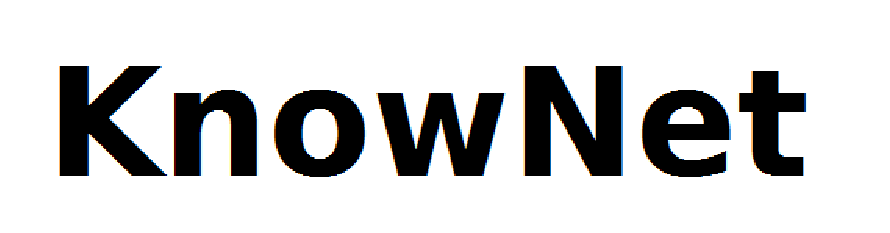
\includegraphics[scale=0.25]{images/knownet_logo}}
\title{KnowNet, eine Ontologie und Suchmaschine f\"ur Dokumente und Statements}
\subject{Idee f\"ur eine Software\\
Piratenpartei Schweiz}

\begin{document}

\maketitle

\newpage
\singlespacing
\tableofcontents

\pagebreak
\onehalfspacing
\setcounter{page}{1}
\pagenumbering{arabic}

\chapter{Einleitung} \label{sec:introduction}

\section{Die Idee \emph{KnowNet}}

\emph{KnowNet} - Knowledge Network - ist prim\"ar eine Ontologie, welche Dokumente von und \"uber ein politische Partei sammelt und entsprechend aufbereitet anbietet. Die Idee dahinter ist, dass man durch eine einfache, eventuell neuartige Suchoberfl\"ache, Aussagen und Meinungen aber auch Dokumente von einer Partei, respektive \"uber eine Partei finden kann. Eine Partei kann rekursiv Untersektionen beinhalten, welche somit bei einem lokalen Thema die Ontologie abfragen k\"onnen, ob zu diesem Thema schon ein Statement oder Dokument vorhanden ist, welche andere Sektion schon etwas dar\"uber gesagt hat, aber auch, ob es eventuell andere Organisatinen wie Medienh\"auser gibt, welche eine Aussage diesbez\"uglich der Partei unterstellt haben.

Die Ontologie soll schlussendlich eine einfache M\"oglichkeit bieten, Dinge \"uber eine komplexe Struktur zu erfahren um daraus Schlussfolgerungen und Thesen auf zu stellen, jedoch auch um heraus zu finden, ob denn schon eine der Sektione eine Meinung oder Uassage \"uber ein gewisses Thema gemacht hat.

\section{Struktur und Aufbau} \label{sec:structure}

Es bietet sich an, \emph{KnowNet} durch eine Ontologie ab zu bilden. Ontologien die auf dem OWL-Standard\cite{W3COWL} basieren, bieten die M\"oglichkeit an, mittels einer in den Grundz\"ugen einfachen Sprache eine Wissensdatenbank komplex verkn\"upft zu speichern und darauf Abfragen aus zu f\"uhren. OWL ist eine Erweiterung von RDF/S und ist wie dieses durch die zwei Syntaxen \emph{Turtle} respektive \emph{N3} und \emph{XML} definiert. Obwohl \emph{XML} im Vergleich zu \emph{Turtle} einiges mehr ''drum herum'' hat, ist es dennoch einfacher zu erstellen und auch zu pflegen denn \emph{Turtle}. Auch kann die Ontologie in dieser Syntak durch andere Programme einfacher gelesen werden und ist auch einfacher wartbar, da Syntaxfehler durch gute Editoren schneller erkennt werden.

OWL ist zur Zeit in Version 1 und in Version 2 definiert. Der OWL 2 Standard\cite{W3COWL2} ist komplett R\"uckw\"artskompatibel zu OWL 1, enth\"allt jedoch Erweiterungen, welche in der Ursprungsversion schlicht gefehlt haben. Einige der Neuerungen sind schlicht syntaktischer Natur, andere sind funktionen und Features welche bislang gefehlt haben. Die Ontologie f\"ur \emph{KnowNet} wird noch mit OWL 1 implementiert, wenn jedoch die verwendeten Libraries (siehe \nameref{sec:technologies} auf Seite \pageref{sec:technologies}) kann diese auch nach OWL 2 konvertiert, respektive deren Neuerungen verwendet werden.

\subsection{Technologien} \label{sec:technologies}

Es werden Folgende Technologien und Standards verwendet:

\begin{description}
  \item[Ontologie] OWL 1, Subsprache OWL DL (Description Logic), als Ontologiebeschreibungssprache
  \item[Abfrage] SPARQL\cite{SPARQL} zur Abfrage
  \item[Programmierung] C/C++ mit Qt4\cite{QT}
  \item[Eventuell] HTML 5, Javascript als Client oder zur Abfrage mittels REST
  \item[Libraries] Redland RDF Libraries\cite{LIBRDF}
  \item[Datenbank] PostgreSQL und MySQL Serverseitig, SQLite zum Entwickeln und eventuell auf dem Client wenn notwendig
\end{description}

Die Liste ist offen und wird entsprechend angepasst wenn bei der Entwicklung und/oder Planung gemerkt wird, dass andere Dinge und Libraries eingesetzt oder nicht verwendet werden.

\chapter{Aufbau der Ontologie} \label{sec:ontology}

% ========== CLASSES ==========

\section{Klassen} \label{sec:class}

Folgende Klassen und Spezialisierungen werden f\"ur die Ontologie gebraucht. In den nachfolgenden Kapiteln werden diese noch genauer beschrieben. Die Verlinkungen zwischen den einzelnen Klassen, also die ObjectProperties, werden im Kapitel \nameref{sec:relations} auf Seite \pageref{sec:relations} beschrieben. In den jeweiligen Detailbeschreibungen der Klassen wird jeweils darauf eingegangen und darauf verwiesen. Die Datenfelder, also die DataProperties, werden in den Detailbeschreibungen der Klassen beschrieben.

\begin{itemize}
  \item Thing
  \begin{itemize}
    \item Word
    \item Sentence
    \item Translation
    \item Synonym
    \item Document
    \begin{itemize}
      \item Paper
      \item Statement
      \item Journal
    \end{itemize}
    \item Person
    \item Profession
    \item Organization
    \item Association
  \end{itemize}
\end{itemize}

\begin{table}[H]
  \centering
  \begin{tabular}{ | l | p{4cm} | l | l| }
    \hline
    \textbf{Class} & \textbf{Beschreibung} & \textbf{SubClass of} & \textbf{Details} \\ \hline
    \textbf{Word} & Beschreibt ein einzelnes Wort in einer Sprache, es kann auch aus mehreren w\"ortern zusammengesetzt sein; Anhand einer ID kann ein Link zu einer anderen Sprache oder einenmSynonym hergestellt werden; & Thing & \nameref{sec:class_word} auf Seite \pageref{sec:class_word} \\ \hline
    \textbf{Translation} & Gruppiert die gleichen W\"orter aus verschiedenen Sprachen & Thing & \nameref{sec:class_translation} auf Seite \pageref{sec:class_translation} \\ \hline
    \textbf{Synonym} & Gruppiert unterschiedliche W\"orter der gleichen Sprache mit der gleichen Bedeutung & Thing & \nameref{sec:class_synonym} auf Seite \pageref{sec:class_synonym} \\ \hline
    \textbf{Sentence} & Ein Satz besteht aus verschiedenen W\"ortern & Thing & \nameref{sec:class_sentence} auf Seite \pageref{sec:class_sentence} \\ \hline
    \textbf{Document} & Ein Dokument ist eine Sammlung von S\"atzen inkl. einigen weiteren Attributen & Thing & \nameref{sec:class_document} auf Seite \pageref{sec:class_document} \\ \hline
    \textbf{Paper} & Ein Positionspapier oder eine andere Dokumentation einer Partei & Document & \nameref{sec:class_paper} auf Seite \pageref{sec:class_paper} \\ \hline
    \textbf{Statement} & Eine Aussage, welche ein Mitglied einer Partei gemacht hat und welche so vertreten wird & Document & \nameref{sec:class_statement} auf Seite \pageref{sec:class_statement} \\ \hline
    \textbf{Journal} & Ein Zeitungsbericht & Document & \nameref{sec:class_journal} auf Seite \pageref{sec:class_journal} \\ \hline
    \textbf{Person} & Eine Person im Allgemeinen & Thing & \nameref{sec:class_person} auf Seite \pageref{sec:class_person} \\ \hline
    \textbf{Profession} & Beschreibt einen Beruf, welcher eine Person aus\"uben kann & Person & \nameref{sec:class_profession} auf Seite \pageref{sec:class_profession} \\ \hline
    \textbf{Organization} & Eine Organisation/Medienhaus welches Zeitungen etc. herstellt, Arbeitgeber eines Journalisten & Thing & \nameref{sec:class_organization} auf Seite \pageref{sec:class_organization} \\ \hline
    \textbf{Association} & Eine (politische) Partei, welche Mitglieder und Angestellte hat & Thing & \nameref{sec:class_association} auf Seite \pageref{sec:class_association} \\ \hline
  \end{tabular}
  \caption{Kurze Beschreibung der Klassen in der Ontologie}
  \label{tbl:classes}
\end{table}


\subsection{Klasse: Word} \label{sec:class_word}

Die Klasse \emph{Word} wird verwendet, um ein einzelnes Wort, welches innerhalb eines Dokumentes gefunden werden soll, zu definieren. Einzelne W\"orter k\"onnen mit der Relation \emph{wordcombo} (siehe \nameref{sec:rel_wordcombo} Seite \pageref{sec:rel_wordcombo}) zu Wortkombinationen zusammengesetzt werden. Durch das Datenfeld \emph{language} wird die Sprache des jeweiligen Wortes in iso639-1 (zwei Zeichen) definiert. Um \"Ubersetzungen miteinander zu verkn\"upfen, wird die Klasse \emph{Translation} (siehe \nameref{sec:class_translation} Seite \pageref{sec:class_translation}) verwendet. Durch die Relation \emph{wordtype} wird die Art des Wortes definiert, also ob es sich um ein Nomen, ein Adjektiv oder ein Verb handelt.

\subsubsection{Code}  \label{sec:class_word_code}

\begin{figure}[H]
 \lstset{language=XML}
 \begin{lstlisting}[label=owl:word,caption={Die Klasse \emph{Word} beschreibt ein einzelnes Wort}]
<owl:Class rdf:ID="#Word">
</owl:Class>
 \end{lstlisting}
\end{figure}

\subsection{Klasse: Translation} \label{sec:class_translation}

Die Klasse \emph{Translation} ist eine Vereinigung aller W\"orter verschiedener Sprachen mit der selben Bedeutung. Dies geschieht durch das Konstrukt \texttt{owl:oneOf} und der Angabe aller Individuen. Durch dieses Konstrukt k\"onnen neue W\"orter einfach und schnell eingepflegt und \"ubersetzt werden und bei einer Abfrage kann jeweils eines aus der Liste gesucht werden.

\subsubsection{Code}  \label{sec:class_translation_code}

\begin{figure}[H]
 \lstset{language=XML}
 \begin{lstlisting}[label=owl:translation,caption={Die Klasse \emph{Translation} beinhaltet alle \"Ubersetzungen eines Wortes}]
<owl:Class rdf:ID="#Translation">
  <owl:oneOf rdf:parseType="Collection">
    <Word rdf:about="#Word_Instance_1" />
    <Word rdf:about="#Word_Instance_2" />
    ...
  </owl:oneOf>
</owl:Class>
 \end{lstlisting}
\end{figure}

\subsection{Klasse: Synonym} \label{sec:class_synonym}

Die Klasse \emph{Synonym} dient zur Verkettung von W\"ortern mit der gleichen Bedeutung. Dies geschieht durch das Konstrukt \texttt{owl:oneOf} und der Angabe aller Individuen. Durch dieses Konstrukt k\"onnen neue W\"orter einfach und schnell eingepflegt und als Synonyme definiert werden, sowie bei einer Abfrage in der Liste gesucht werden.


\subsubsection{Code}  \label{sec:class_synonym_code}

\begin{figure}[H]
 \lstset{language=XML}
 \begin{lstlisting}[label=owl:synonym,caption={Die Klasse \emph{Synonym} beinhaltet alle W\"orter dir etwas \"ahnliches bedeuten}]
<owl:Class rdf:ID="#Synonym">
  <owl:oneOf rdf:parseType="Collection">
    <Word rdf:about="#Word_Instance_1" />
    <Word rdf:about="#Word_Instance_2" />
    ...
  </owl:oneOf>
</owl:Class>
 \end{lstlisting}
\end{figure}

\subsection{Klasse: Sentence} \label{sec:class_sentence}

Ein Satz, welcher durch die Klasse \emph{Sentence} definiert wird, ist eine Vereinigung von W\"ortern zu einer Gruppe von solchen. Die Reihenfolge der W\"orter ist hierbei egal, es geht nur um das Zusammenspiel und den Zusammenhang einzelner W\"orter. Dieses Konstrukt wird bei der Instanz im Property \emph{has-word} (siehe \nameref{sec:rel_hasword} Seite \pageref{sec:rel_hasword}) durch eine anonyme Klasse mit \texttt{owl:unionOf} definiert.

\subsubsection{Code}  \label{sec:class_sentence_code}

\begin{figure}[H]
 \lstset{language=XML}
 \begin{lstlisting}[label=owl:sentence,caption={Die Klasse \emph{Sentence} f\"ugt einzelne W\"orter zu einem Satz zusammen}]
<owl:Class rdf:ID="#Sentence">
  <rdfs:subClassOf>
    <owl:Restriction>
      <owl:onProperty rdf:resource="#has-word" />
      <owl:someValuesFrom ref:resource="#Word" />
    </owl:Restriction>
  </rdfs:subClassOf>
</owl:Class>
 \end{lstlisting}
\end{figure}

\subsection{Klasse: Document} \label{sec:class_document}

Die Klasse \emph{Document} ist, \"ahnlich wie \emph{Sentence}, eine Kombination von verschiedenen S\"atzen. Die Reihenfolge dieser spielt keine Rolle, es geht rein um den Logischen Zusammenhang der einzelnen S\"atze und somit der verschiedenen W\"orter.

\textit{Anmerkung:} Eventuell macht es hier Sinn, ein Dokument noch durch Kapitel zu strukturieren. Dies kann durch die Relation ''ein Dokument aus Dokumenten'' gemacht werden.

\subsubsection{Code}  \label{sec:class_sentence_code}

\begin{figure}[H]
 \lstset{language=XML}
 \begin{lstlisting}[label=owl:document,caption={Die Klasse \emph{Document} f\"ugt einzelne S\"atze zu einem Dokument zusammen}]
<owl:Class rdf:ID="#Document">
  <rdfs:subClassOf>
    <owl:Restriction>
      <owl:onProperty rdf:resource="#has-sentence" />
      <owl:someValuesFrom ref:resource="#Sentence" />
    </owl:Restriction>
  </rdfs:subClassOf>
</owl:Class>
 \end{lstlisting}
\end{figure}


\subsection{Klasse: Paper} \label{sec:class_paper}

Die Klasse \emph{Paper} ist eine Unterklasse von \emph{Document} und definiert ein Dokument, welches im Zusammenhang zu einem Verein, also der Klasse \emph{Association} steht. Durch diese Unterklasse kann besser nach Dokumenten gesucht werden, welche von einer bestimmten politischen Partei oder einer Sektion von dieser, verfasst wurden. Ein Dokument, welches durch diese Klasse implementiert ist, beschreibt in den meisten F\"allen ein Positionspapier oder \"ahnliches.

\subsubsection{Code} \label{sec:class_paper_code}

\begin{figure}[H]
 \lstset{language=XML}
 \begin{lstlisting}[label=owl:paper,caption={Die Klasse \emph{Paper} ist ein Dokument einer \emph{Association}, also eines partei/Gesellschaft}]
<owl:Class rdf:ID="#Paper">
  <rdfs:subClassOf rdf:resurce="#Document" />
</owl:Class>
 \end{lstlisting}
\end{figure}


\subsection{Klasse: Statement} \label{sec:class_statement}

Die Klasse \emph{Statement} ist eine Unterklasse von \emph{Document} und wird verwendet, um eine Aussage/Statement einer Person zu definieren. Bei einem Statement muss bei der Suche unterschieden werden, ob dieses von einer Person aus der Klasse \emph{Association} stammt, oder von einer beliebigen anderen Person. Ein Statement von einer beliebigen Person kann genutzt werden, um sich ein Bild von Aussen zu machen, w\"ahrend eines von einer Person aus \emph{Association} genutzt werden kann, um sich ein Bild von innen zu machen.

Durch das Property \emph{from-text} (siehe \nameref{sec:res_fromtext} auf Seite \pageref{sec:res_fromtext}) kann ein Statement einem beliebigen anderen \emph{Document} zugeordnet werden.

\subsubsection{Code} \label{sec:class_statement_code}

\begin{figure}[H]
 \lstset{language=XML}
 \begin{lstlisting}[label=owl:statement,caption={Ein \emph{Statement} beschreibt eine Aussage einer Person}]
<owl:Class rdf:ID="#Statement">
    <rdfs:subClassOf rdf:resource="#Document" />
</owl:Class>
 \end{lstlisting}
\end{figure}

\subsection{Klasse: Journal} \label{sec:class_journal}

Ein \emph{Journal} ist eine Unterklasse von \emph{Document} und definiert einen Text, welcher von einem \emph{Writer} oder \emph{Blogger} geschrieben und Ver\"offentlicht worden ist. Er stellt nicht eine Meinung der \emph{Association} dar, sondern diejenige eines Aussenstehenden. Ist der Author ebenfalls Mitglied der Klasse \emph{Member}, kann der Text als pers\"onliche Meinung und somit indirekt als Parteimeinung gedeutet werden.

\subsubsection{Code} \label{sec:class_journal_code}

\begin{figure}[H]
 \lstset{language=XML}
 \begin{lstlisting}[label=owl:journal,caption={Ein \emph{Journal} ist ein Bericht \"uber eine \emph{Association}, welcher von einer \emph{Organization} herausgegeben wurde}]
<owl:Class rdf:ID="#Journal">
  <rdfs:subClassOf rdf:resource="#Document" />
</owl:Class>
 \end{lstlisting}
\end{figure}

\subsection{Klasse: Person} \label{sec:class_person}

Die Klasse \emph{Person} wird verwendet, um irgend eine Person zu definieren. Dies kann ein Autor, ein Parteimitglied oder eine andere beliebige Person sein.

\subsubsection{Code} \label{sec:class_person_code}

\begin{figure}[H]
 \lstset{language=XML}
 \begin{lstlisting}[label=owl:person,caption={Die Klasse \emph{Person} definiert alle Personen}]
<owl:Class rdf:ID="#Person">
</owl:Class>
 \end{lstlisting}
\end{figure}


\subsection{Klasse: Profession} \label{sec:class_profession}

Die Klasse \emph{Profession} wird verwendet, um einer \emph{Person} einen Beruf/Anstellung zuzuweisen. Dadurch kann man gegebenenfalls gewissen Berufsgruppen gewissen Meinungen zuweisen.

Die Zuweisung erfolgt durch die Relation \emph{working-as} (siehe \nameref{sec:rel_workingas} auf Seite \pageref{sec:rel_workingas}).

\subsubsection{Code} \label{sec:class_profession_code}

\begin{figure}[H]
 \lstset{language=XML}
 \begin{lstlisting}[label=owl:profession,caption={Die Klasse \emph{Caption} beschreibt jegliche Berufe}]
<owl:Class rdf:ID="#Profession">
  <rdfs:subClassOf>
    <owl:Restriction>
      <owl:onProperty rdf:resource="#has-workers" />
      <owl:someValuesFrom ref:resource="#Person" />
    </owl:Restriction>
  </rdfs:subClassOf>
</owl:Class>
 \end{lstlisting}
\end{figure}


\subsection{Klasse: Organization} \label{sec:class_organization}

Die Klasse \emph{Organization} definiert den Arbeitgeber von einer \emph{Person}. Durch diese Zuweisung k\"onnen Aussagen und Meinungen, welche eine Zeitung von der Partei hat, eruiert werden. Eine \emph{Organization} kann mehrere Angestellte haben, welche nicht zwingendermassen nur bei der einen Organisation angestellt sind. Idealerweise besitzt die \emph{Person} ebenfalls das Attribut \emph{working-as} mit enem Verweis auf einen Beruf.

Eine Instanz kann nie gleichzeitig eine \emph{Organization} und eine \emph{Association} sein, diese zwei Klassen schliessen sich gegenseitig aus.

\subsubsection{Code} \label{sec:class_organization_code}

\begin{figure}[H]
 \lstset{language=XML}
 \begin{lstlisting}[label=owl:organization,caption={Die Klasse \emph{Organization} definiert einen Arbeitgeben, meistens ein Medienhaus}]
<owl:Class rdf:ID="#Organization">
  <rdfs:subClassOf>
    <owl:Restriction>
      <owl:onProperty rdf:resource="#has-employee" />
      <owl:someValuesFrom ref:resource="#Person" />
    </owl:Restriction>
  </rdfs:subClassOf>
  <owl:disjointWith rdf:resource="#Association" />
</owl:Class>
 \end{lstlisting}
\end{figure}


\subsection{Klasse: Association} \label{sec:class_association}

Eine \emph{Association} definiert eine Politische Partei oder andere Gesellschaft, \"uber welche man sich durch diese Ontologie ein Bild verschaffen k\"onnen soll.

Eine Instanz kann nie gleichzeitig eine \emph{Organization} und eine \emph{Association} sein, diese zwei Klassen schliessen sich gegenseitig aus.

\subsubsection{Code} \label{sec:class_association_code}

\begin{figure}[H]
 \lstset{language=XML}
 \begin{lstlisting}[label=owl:association,caption={Eine \emph{Association} ist eine politische Partei oder eine andere Gesellschaft}]
<owl:Class rdf:ID="#Association">
  <rdfs:subClassOf>
    <owl:Restriction>
      <owl:onProperty rdf:resource="#has-member" />
      <owl:someValuesFrom ref:resource="#Member" />
    </owl:Restriction>
  </rdfs:subClassOf>
  <owl:disjointWith rdf:resource="#Organization" />
</owl:Class>
 \end{lstlisting}
\end{figure}


% ========== RELATIONS ==========

\section{Relationen} \label{sec:reltations}

Die Relationen, resp. Properties, beschreiben die Abh\"angigkeiten wie auch die Verkn\"upfungen unter den Klassen. Relationen, welche klassenspezifisch sind, also direkt gebraucht werden um eine Klasse zu beschreiben, sind als anonyme Unterklassen bereits in diesen definiert worden. Hier werden nur diejenigen Relationen beschrieben, welche verwendet werden zur direkten dynamischen und individuellen Verkn\"upfung verschiedener Instanzen.

\begin{table}[H]
  \centering
  \begin{tabular}{ | l | p{4cm} | p{3cm} | p{2cm} | p{2cm} | }
    \hline
    \textbf{Relation} & \textbf{Beschreibung} & \textbf{Domain} & \textbf{Range} & \textbf{Details} \\ \hline
    \textbf{refers-to} & Beziehung zwischen einzenlnen Dokumenten & \emph{Document} & \emph{Document} & \nameref{sec:rel_refersto} auf Seite \pageref{sec:rel_refersto} \\ \hline
    \textbf{has-sentence} & Gibt an, aus welchen S\"atzen ein Dokument besteht & \emph{Document} & \emph{Sentence} & \nameref{sec:rel_hassentence} auf Seite \pageref{sec:rel_hassentence} \\ \hline
    \textbf{sentence-of} & Gibt an, in welchem Dokuemnt dieser Satz vorhanden ist & \emph{Sentence} & \emph{Document} & \nameref{sec:rel_sentenceof} auf Seite \pageref{sec:rel_sentenceof} \\ \hline
    \textbf{has-word} & Gibt an, aus welchen W\"ortern ein Satz besteht & \emph{Sentence} & \emph{Word} & \nameref{sec:rel_hasword} auf Seite \pageref{sec:rel_hasword} \\ \hline
    \textbf{word-of} & Gibt an, in welchem Satz ein Wort vorhanden ist & \emph{Word} & \emph{Sentence} & \nameref{sec:rel_wordof} auf Seite \pageref{sec:rel_wordof} \\ \hline
    \textbf{combined-in} & Gibt an, dass ein Wort mit einem anderen verkn\"upft werden kann & \emph{Word} & \emph{Word} & \nameref{sec:rel_wordcombo} auf Seite \pageref{sec:rel_wordcombo} \\ \hline
    \textbf{has-writer} & Definiert einen oder mehrere Autoren eines Dokuments & \emph{Document} & \emph{Person} & \nameref{sec:rel_haswriter} auf Seite \pageref{sec:rel_haswriter} \\ \hline
    \textbf{writer-of} & Definiert die Dokumente, an welchen eine Person mitgearbeitet hat & \emph{Person} & \emph{Document} & \nameref{sec:rel_writerof} auf Seite \pageref{sec:rel_writerof} \\ \hline
    \textbf{has-subregion} & Definiert die Sub-Associations der aktuellen & \emph{Association} & \emph{Association} & \nameref{sec:rel_hassubregion} auf Seite \pageref{sec:rel_hassubregion} \\ \hline
    \textbf{subregion-of} & Definiert, dass diese Association eine Sub-Association der angegebenen ist & \emph{Association} & \emph{Association} & \nameref{sec:rel_subregionof} auf Seite \pageref{sec:rel_subregionof} \\ \hline
  \end{tabular}
  \caption{Kurze Beschreibung der Relationen in der Ontologie}
  \label{tbl:classes}
\end{table}

\begin{table}[H]
  \centering
  \begin{tabular}{ | l | p{4cm} | p{3cm} | p{2cm} | p{2cm} | }
    \hline
    \textbf{Relation} & \textbf{Beschreibung} & \textbf{Domain} & \textbf{Range} & \textbf{Details} \\ \hline
    \textbf{has-employee} & Gibt alle Employees der Organization an & \emph{Organization}, \emph{Association} & \emph{Employee} & \nameref{sec:rel_hasemployee} auf Seite \pageref{sec:rel_hasemployee} \\ \hline
    \textbf{employee-of} & Gibt an, bei welchen Organizations der Employee angestellt ist & \emph{Employee} & \emph{Organization}, \emph{Association} & \nameref{sec:rel_employeeof} auf Seite \pageref{sec:rel_employeeof} \\ \hline
    \textbf{has-member} & Definiert alle Mitglieder einer Association & \emph{Association} & \emph{Member} & \nameref{sec:rel_hasmember} auf Seite \pageref{sec:rel_hasmember} \\ \hline
    \textbf{member-of} & Definiert in welcher Association der Member Mitglied ist & \emph{Member} & \emph{Association} & \nameref{sec:rel_memberof} auf Seite \pageref{sec:rel_memberof} \\ \hline
    \textbf{has-document} & gibt an, welche Associaton oder Organization ein dokument verfasst hat & \emph{Association}, \emph{Organization} & \emph{Document} & \nameref{sec:rel_hasdocument} auf Seite \pageref{sec:rel_hasdocument} \\ \hline
    \textbf{document-of} & gibt an, zu welcher Association oder Organization ein Dokument geh\"ort & \emph{Document} & \emph{Association}, \emph{Organization} & \nameref{sec:rel_documentof} auf Seite \pageref{sec:rel_documentof} \\ \hline
    \textbf{is-about} & Definiert, dass das aktuelle Dokument etwas \"uber die angegebene Assoiciation aussagt & \emph{Document} & \emph{Association} & \nameref{sec:rel_isabout} auf Seite \pageref{sec:rel_isabout} \\ \hline
    \textbf{mentioned-in} & Gibt an, in welchem Dokument auf die Association referenziert wird & \emph{Association} & \emph{Document} & \nameref{sec:rel_mentionedin} auf Seite \pageref{sec:rel_mentionedin} \\ \hline
  \end{tabular}
  \caption{Kurze Beschreibung der Relationen in der Ontologie}
  \label{tbl:classes}
\end{table}

\subsubsection{M\"ogliche Eigenschaften} \label{sec:relations_settings}

Relationen k\"onnen folgende Charakteristiken aufweisen:

\begin{description}
  \item[Funktional] Eine funktionale Relation \texttt{P} impliziert: \\
    wenn \texttt{P(u, v)} und \texttt{P(u, w)} dann \texttt{v == w}
  \item[Invers Funktional] Eine inverse funktionale Relation \texttt{P} impliziert: \\
    wenn \texttt{P(v, u)} und \texttt{P(w, u)} dann \texttt{v == w}
  \item[Transitiv] Wenn eine Relation \texttt{P} \emph{transitiv} definiert ist f\"ur \texttt{u, v, w}: \\
    wenn \texttt{P(u, v)} und \texttt{P(v, w)} impliziert \texttt{P(u, w)}
  \item[Symmetrisch] Wenn eine Relation \texttt{P} symmetrisch definiert ist: \\
    wenn \texttt{P(u, v)} dann \texttt{P(v, u)}
  \item[InverseOf] Wenn bei der Relation \texttt{P1} eine Inverse Relation \texttt{P2} definiert ist:\\
    wenn \texttt{P1(u, v)} dann \texttt{P2(v, u)}
\end{description}

\textbf{Wichtig}: Die Eigenschaften \emph{Reflexiv}, \emph{Irreflexiv} und \emph{Asymmetrisch} aus der OWL-2 Definition werden nicht verwendet.


\subsection{Relation: refers-to} \label{sec:rel_refersto}

Die Relation \emph{refers-to} beschreibt die Beziehungen zwischen den einzelnen Dokumenten. Wird zum Beispiel in einem Blog, was ja als \emph{Document} interpertiert ist, auf einen Artikel uas einer Zeitung verwiesen, so kann dies durch diese Relation definiert werden. Die Relation ist sowohl \emph{symmetrisch} als auch \emph{transitiv} und das inverse von sich selbst.

\subsubsection{Eigenschaften} \label{sec:rel_refersto_settings}

\begin{itemize}
  \item Transitiv
  \item Symmetrisch
  \item inverseOf \emph{refers-to}
\end{itemize}

\subsubsection{Code} \label{sec:rel_refersto_code}

\begin{figure}[H]
 \lstset{language=XML}
 \begin{lstlisting}[label=owl:refersto,caption={Die Relation \emph{refers-to} beschreibt die Abh\"angigkeiten unter Dokumenten}]
<owl:ObjectProperty rdf:ID="#refers-to">
  <rdf:type rdf:resource="&owl;TransitiveProperty" />
  <rdf:type rdf:resource="&owl;SymmetricProperty" />
  <owl:inverseOf rdf:resource="#refers-to" />
  <rdfs:domain rdf:resource="#Document" />
  <rdfs:range rdf:resource="#Document" />
</owl:ObjectProperty>
 \end{lstlisting}
\end{figure}


\subsection{Relation: has-sentence} \label{sec:rel_hassentence}

Die Relation \emph{has-sentence} gibt an, welche \emph{Sentence} Instanzen in einem \emph{Document} vorkommen.

\subsubsection{Eigenschaften} \label{sec:rel_hassentence_settings}

\begin{itemize}
  \item inverseOf \emph{sentence-of}
\end{itemize}

\subsubsection{Code} \label{sec:rel_hassentence_code}

\begin{figure}[H]
 \lstset{language=XML}
 \begin{lstlisting}[label=owl:hassentence,caption={Die Relation \emph{has-sentence} gibt an, welches Dokuemnt aus welchen S\"atzen besteht}]
<owl:ObjectProperty rdf:ID="#has-sentence">
  <rdfs:domain rdf:resource="#Document" />
  <rdfs:range rdf:resource="#Sentence" />
</owl:ObjectProperty>
 \end{lstlisting}
\end{figure}


\subsection{Relation: sentence-of} \label{sec:rel_sentenceof}

Die Relation \emph{sentence-of} gibt an, in welchem \emph{Document} ein \emph{Sentence} vorkommt.

\subsubsection{Eigenschaften} \label{sec:rel_sentenceof_settings}

\begin{itemize}
  \item Transitiv
  \item inverseOf \emph{has-sentence}
\end{itemize}

\subsubsection{Code} \label{sec:rel_sentenceof_code}

\begin{figure}[H]
 \lstset{language=XML}
 \begin{lstlisting}[label=owl:sentenceof,caption={Die Relation \emph{sentenceof} gibt an, in welchem Dokument ein Satz vorkommt}]
<owl:ObjectProperty rdf:ID="#sentence-of">
  <rdfs:domain rdf:resource="#Sentence" />
  <rdfs:range rdf:resource="#Document" />
</owl:ObjectProperty>
 \end{lstlisting}
\end{figure}


\subsection{Relation: has-word} \label{sec:rel_hasword}

Die Relation \emph{has-word} gibt an, welche \emph{Word} Instanz in der \emph{Sentence} Instanz verwendet wird. Die Reihenfolge der W\"orter in den S\"atzen spielt keine rolle, es kommt nur auf den Sinn der W\"orter an.

\subsubsection{Eigenschaften} \label{sec:rel_hasword_settings}

\begin{itemize}
  \item Transitiv
  \item inverseOf \emph{word-of}
\end{itemize}

\subsubsection{Code} \label{sec:rel_hasword_code}

\begin{figure}[H]
 \lstset{language=XML}
 \begin{lstlisting}[label=owl:hasword,caption={Die Relation \emph{has-word} gibt an, welches Wort in einem Satz vorkommt}]
<owl:ObjectProperty rdf:ID="#has-word">
  <rdfs:domain rdf:resource="#Sentence" />
  <rdfs:range rdf:resource="#Word" />
</owl:ObjectProperty>
 \end{lstlisting}
\end{figure}


\subsection{Relation: word-of} \label{sec:rel_wordof}

Die Relation \emph{word-of} gibt an, in welchen \emph{Sentence} Instanzen ein \emph{Word} verwendet wird. Die Reihenfolge der W\"ortern in den S\"atzen spielt keine Rolle, es kommt nur auf den Sinn der W\"orter an.

\subsubsection{Eigenschaften} \label{sec:rel_wordof_settings}

\begin{itemize}
  \item Transitiv
  \item inverseOf \emph{has-word}
\end{itemize}

\subsubsection{Code} \label{sec:rel_wordof_code}

\begin{figure}[H]
 \lstset{language=XML}
 \begin{lstlisting}[label=owl:wordof,caption={Die Relation \emph{word-of} gibt an, in welchem Satz das Wort vorkommt}]
<owl:ObjectProperty rdf:ID="#word-of">
  <rdfs:domain rdf:resource="#Word" />
  <rdfs:range rdf:resource="#Sentence" />
</owl:ObjectProperty>
 \end{lstlisting}
\end{figure}


\subsection{Relation: has-writer} \label{sec:rel_haswriter}

Die Relation \emph{has-writer} definiert alle \emph{Person} Instanzen, welche an dem aktuellen \emph{Document} gearbeitet haben.

\subsubsection{Eigenschaften} \label{sec:rel_haswriter_settings}

\begin{itemize}
  \item Transitiv
  \item inverseOf \emph{writer-of}
\end{itemize}

\subsubsection{Code} \label{sec:rel_haswriter_code}

\begin{figure}[H]
 \lstset{language=XML}
 \begin{lstlisting}[label=owl:haswriter,caption={Die Relation \emph{has-writer} gibt an, welche \emph{Person} an dem \emph{Document} geschrieben hat}]
<owl:ObjectProperty rdf:ID="#has-writer">
  <rdfs:domain rdf:resource="#Document" />
  <rdfs:range rdf:resource="#Person" />
</owl:ObjectProperty>
 \end{lstlisting}
\end{figure}


\subsection{Relation: writer-of} \label{sec:rel_writerof}

Die Relation \emph{writer-of} definiert die Verlinkung einer \emph{Person} mit einem \emph{Document}. Daraus kann gelesen werden, welche Person welches Dokument erstellt, respektive daran mitgearbeitet hat.

\subsubsection{Eigenschaften} \label{sec:rel_writerof_settings}

\begin{itemize}
  \item Transitiv
  \item inverseOf \emph{has-writer}
\end{itemize}

\subsubsection{Code} \label{sec:rel_writerof_code}

\begin{figure}[H]
 \lstset{language=XML}
 \begin{lstlisting}[label=owl:writerof,caption={Die Relation \emph{writer-of} gibt an, welche \emph{Person} an welchem \emph{Document} gearbeitet hat}]
<owl:ObjectProperty rdf:ID="#writer-of">
  <rdfs:domain rdf:resource="#Person" />
  <rdfs:range rdf:resource="#Document" />
</owl:ObjectProperty>
 \end{lstlisting}
\end{figure}


\subsection{Relation: has-subregion} \label{sec:rel_hassubregion}

Die Relation \emph{has-subregion} definiert alle \emph{Association} Instanzen, welche unterhalb der aktiven angelegt sind. Instanzen von \emph{Association} k\"onnen in einer Baumstruktur angeordnet werden. Diese Property definiert die Verlinkung von Oben nach Unten.

\subsubsection{Eigenschaften} \label{sec:rel_hassubregion_settings}

\begin{itemize}
  \item Transitiv
  \item Inverse Funktional
  \item inverseOf \emph{subregion-of}
\end{itemize}

\subsubsection{Code} \label{sec:rel_hassubregion_code}

\begin{figure}[H]
 \lstset{language=XML}
 \begin{lstlisting}[label=owl:hassubregion,caption={Die Relation \emph{has-subregion} definiert, welche Untersektionen eine \emph{Association} hat}]
<owl:ObjectProperty rdf:ID="#has-subregion">
  <rdfs:domain rdf:resource="#Association" />
  <rdfs:range rdf:resource="#Association" />
</owl:ObjectProperty>
 \end{lstlisting}
\end{figure}


\subsection{Relation: subregion-of} \label{sec:rel_subregionof}

Die Relation \emph{subregion-of} definiert die Eltern-Instanz der aktiven \emph{Association} Instanz. Instanzen von \emph{Association} k\"onnen in einer Baumstruktur angeordnet werden. Dieses Property definiert die Verlinkung von einer Unten nach Oben.

\subsubsection{Eigenschaften} \label{sec:rel_subregionof_settings}

\begin{itemize}
  \item Transitiv
  \item inverseOf \emph{has-subregion}
\end{itemize}

\subsubsection{Code} \label{sec:rel_subregionof_code}

\begin{figure}[H]
 \lstset{language=XML}
 \begin{lstlisting}[label=owl:subregionof,caption={Die Relation \emph{subregion-of} definiert die \"ubergeordnete \emph{Association}}]
<owl:ObjectProperty rdf:ID="#subregion-of">
  <rdfs:domain rdf:resource="#Association" />
  <rdfs:range rdf:resource="#Associaton" />
</owl:ObjectProperty>
 \end{lstlisting}
\end{figure}


\subsection{Relation: has-employee} \label{sec:rel_hasemployee}

Die Relation \emph{has-employee} definiert alle \emph{Person} Instanzen, welche bei der gegebenen \emph{Organization} oder \emph{Assocaition} arbeiten. Eine \emph{Person} kann bei mehreren \emph{Organization} angestellt sein.

\subsubsection{Eigenschaften} \label{sec:rel_hasemployee_settings}

\begin{itemize}
  \item Transitiv
  \item inverseOf \emph{employee-of}
\end{itemize}

\subsubsection{Code} \label{sec:rel_hasemployee_code}

\begin{figure}[H]
 \lstset{language=XML}
 \begin{lstlisting}[label=owl:hasemployee,caption={Die Relation \emph{has-employee} gibt an, welche \emph{Person} bei der \emph{Organization} oder \emph{Association} angestellt sind}]
<owl:ObjectProperty rdf:ID="#has-employee">
  <rdfs:domain>
    <owl:Class>
      <owl:unionOf rdf:parseType="Collection">
        <owl:Class rdf:about="#Organization" />
        <owl:Class rdf:about="#Association" />
      </owl:unionOf>
    </owl:Class>
  </rdfs:domain>
  <rdfs:range rdf:resource="#Person" />
</owl:ObjectProperty>
 \end{lstlisting}
\end{figure}


\subsection{Relation: employee-of} \label{sec:rel_employeeof}

Die Relation \emph{employee-of} weisst einer \emph{Person} einen Arbeitgeber zu. Eine \emph{Person}, welche eine solche Zuweisung aufweist, sollte entsprechend auch über die Relation \emph{working-as} verf\"ugen, um so zu definieren, welchen Beruf diese Person aus\"ubt.

Der Arbeitgeber kann entweder eine \emph{Organization} oder aber eine \emph{Association} sein. Eine Person kann mehrere Arbeitgeber aufweisen.

\subsubsection{Eigenschaften} \label{sec:rel_employeeof_settings}

\begin{itemize}
  \item Transitiv
  \item inverseOf \emph{has-employee}
\end{itemize}

\subsubsection{Code} \label{sec:rel_employeeof_code}

\begin{figure}[H]
 \lstset{language=XML}
 \begin{lstlisting}[label=owl:employeeof,caption={Die Relation \emph{employee-of} gibt an, bei welcher \emph{Organization} oder \emph{Association} die Person angestellt ist}]
<owl:ObjectProperty rdf:ID="#employee-of">
  <rdfs:domain rdf:resource="#Person" />
  <rdfs:range>
    <owl:Class>
      <owl:unionOf rdf:parseType="Collection">
        <owl:Class rdf:about="#Organization" />
        <owl:Class rdf:about="#Association" />
      </owl:unionOf>
    </owl:Class>
  </rdfs:range>
</owl:ObjectProperty>
 \end{lstlisting}
\end{figure}


\subsection{Relation: working-as} \label{sec:rel_workingas}

Die Relation \emph{working-as} weisst einer \emph{Person} einen oder mehrere Berufe zu. Durch dieses Property kann beispielsweise gepr\"uft werden, ob gewisse Meinungen oder Richtungen nur in gewissen Berufsgattungen vorherschen, oder ob dies die breitere Masse betrifft.

\subsubsection{Eigenschaften} \label{sec:rel_workingas_settings}

\begin{itemize}
  \item Transitiv
  \item inverseOf \emph{working-as}
\end{itemize}

\subsubsection{Code} \label{sec:rel_workingas_code}

\begin{figure}[H]
 \lstset{language=XML}
 \begin{lstlisting}[label=owl:workingas,caption={Die Relation \emph{working-as} gibt an, welchen Beruf eine Person aus\"ubt}]
<owl:ObjectProperty rdf:ID="#working-as">
  <rdfs:domain rdf:resource="#Person" />
  <rdfs:range rdf:resource="#Profession" />
</owl:ObjectProperty>
 \end{lstlisting}
\end{figure}


\subsection{Relation: has-member} \label{sec:rel_hasmember}

Die Relation \emph{has-member} enth\"allt alle \emph{Person} Instanzen, welche Mitglied bei der gegebenen \emph{Association} sind.

\subsubsection{Eigenschaften} \label{sec:rel_hasmember_settings}

\begin{itemize}
  \item Transitiv
  \item inverseOf \emph{member-of}
\end{itemize}

\subsubsection{Code} \label{sec:rel_hasmember_code}

\begin{figure}[H]
 \lstset{language=XML}
 \begin{lstlisting}[label=owl:ahsmember,caption={Die Relation \emph{has-member} enth\"allt alle Mitglieder der \emph{Association}}]
<owl:ObjectProperty rdf:ID="#has-member">
  <rdfs:domain rdf:resource="#Association" />
  <rdfs:range rdf:resource="#Person" />
</owl:ObjectProperty>
 \end{lstlisting}
\end{figure}


\subsection{Relation: member-of} \label{sec:rel_memberof}

Die Relation \emph{member-of} weisst eine \emph{Person} einer \emph{Association} zu. Dadurch wird definiert, dass diese Person Mitglied der Partei, resp. Gesellschaft ist und deren Meinung offiziell vertreten darf. Eine \emph{Person} kann mehreren \emph{Association} zugewiesen werden.

\subsubsection{Eigenschaften} \label{sec:rel_memberof_settings}

\begin{itemize}
  \item Transitiv
  \item inverseOf \emph{has-member}
\end{itemize}

\subsubsection{Code} \label{sec:rel_memberof_code}

\begin{figure}[H]
 \lstset{language=XML}
 \begin{lstlisting}[label=owl:memberof,caption={Die Relation \emph{member-of} gibt alle \emph{Association} an, bei welcher die Person Mitglied ist}]
<owl:ObjectProperty rdf:ID="#member-of">
  <rdfs:domain rdf:resource="#Person" />
  <rdfs:range rdf:resource="#Association" />
</owl:ObjectProperty>
 \end{lstlisting}
\end{figure}


\subsection{Relation: has-document} \label{sec:rel_hasdocument}

Die Relation \emph{has-document} gibt an, welche \emph{Organization} oder \emph{Association} welches \emph{Document} ver\"offentlicht hat. Das Property beinhaltet in der Domain also entweder eine Instanz einer \emph{Organization} oder einer \emph{Association} und in der Range ein \emph{Document}. Da in der Range unterschiedliche Typen vorkommen k\"onnen, m\"ussen diese in der Klassendefinition (siehe \nameref{sec:class_organization} und \nameref{sec:class_association}) explizit als Unterschiedliche Klassen definiert werden.

\subsubsection{Eigenschaften} \label{sec:rel_hasdocument_settings}

\begin{itemize}
  \item Transitiv
  \item inverseOf \emph{document-of}
\end{itemize}

\subsubsection{Code} \label{sec:rel_hasdocument_code}

\begin{figure}[H]
 \lstset{language=XML}
 \begin{lstlisting}[label=owl:hasdocument,caption={Die Relation \emph{has-document} verkn\"upft eine \emph{Organization} mit einem \emph{Document}}]
<owl:ObjectProperty rdf:ID="#has-document">
  <rdfs:domain>
    <owl:Class>
      <owl:unionOf rdf:parseType="Collection">
        <owl:Class rdf:about="#Organization" />
        <owl:Class rdf:about="#Association" />
      </owl:unionOf>
    </owl:Class>
  </rdfs:domain>
  <rdfs:range rdf:resource="#Document" />
</owl:ObjectProperty>
 \end{lstlisting}
\end{figure}


\subsection{Relation: document-of} \label{sec:rel_documentof}

Die Relation \emph{document-of} gibt an, welche \emph{Organization} oder \emph{Association} der ''Eigent\"umer'' eines Dokumentes ist. Es wird also definiert, wer ein Dokuemnt ver\"offentlicht hat. Das Property beinhaltet demnach in der Domain eine Instanz eines \emph{Document} und in der Range entweder eine \emph{Organization} oder eine \emph{Association}. Da in der Range unterschiedliche Typen vorkommen k\"onnen, m\"ussen diese in der Klassendefinition (siehe \nameref{sec:class_organization} und \nameref{sec:class_association}) explizit als Unterschiedliche Klassen definiert werden.

\subsubsection{Eigenschaften} \label{sec:rel_documentof_settings}

\begin{itemize}
  \item Transitiv
  \item inverseOf \emph{has-document}
\end{itemize}

\subsubsection{Code} \label{sec:rel_documentof_code}

\begin{figure}[H]
 \lstset{language=XML}
 \begin{lstlisting}[label=owl:documentof,caption={Die Relation \emph{document-of} gibt an, welche \emph{Organization} oder \emph{Association} das \emph{Document} ver\"offentlicht hat}]
<owl:ObjectProperty rdf:ID="#document-of">
  <rdfs:domain rdf:resource="#Document" />
  <rdfs:range>
    <owl:Class>
      <owl:unionOf rdf:parseType="Collection">
        <owl:Class rdf:about="#Organization" />
        <owl:Class rdf:about="#Association" />
      </owl:unionOf>
    </owl:Class>
  </rdfs:range>
</owl:ObjectProperty>
 \end{lstlisting}
\end{figure}


\subsection{Relation: is-about} \label{sec:rel_isabout}

Die Relation \emph{is-about} beschreibt, welche \emph{Association} Instanzen im gegebenen \emph{Document} erw\"ahnt wird. Das Property enth\"allt also eine Instanz eines \emph{Document} in der domain und eine Liste von \emph{Association} Instanzen in der Range.

\subsubsection{Eigenschaften} \label{sec:rel_isabout_settings}

\begin{itemize}
  \item Transitiv
  \item inverseOf \emph{mentioned-in}
\end{itemize}

\subsubsection{Code} \label{sec:rel_isabout_code}

\begin{figure}[H]
 \lstset{language=XML}
 \begin{lstlisting}[label=owl:isabout,caption={Die Relation \emph{is-about} gibt an, \"uber welche \emph{Association} ein Dokument ist}]
<owl:ObjectProperty rdf:ID="#is-about">
  <rdfs:domain rdf:resource="#Document" />
  <rdfs:range rdf:resource="#Association" />
</owl:ObjectProperty>
 \end{lstlisting}
\end{figure}


\subsection{Relation: mentioned-in} \label{sec:rel_mentionedin}

Die Relation \emph{mentioned-in} gibt an, in welchen \emph{Document} Instanzen die \emph{Association} erw\"ahnt wird. Das Property enth\"allt also eine Instanz einer \emph{Association} in der Domain und eine Liste von \emph{Document} Instanzen in der Range. Je nach Dokument-Instanz, also der Unterklasse, kann ein internes oder externes Meinungsbild geschaffen werden. Zu beachten ist auch noch das Property \emph{member-of} wie auch \emph{writer-of}, welche die Autoren definieren und deren Parteizugeh\"origkeit.

\subsubsection{Eigenschaften} \label{sec:rel_mentionedin_settings}

\begin{itemize}
  \item Transitiv
  \item inverseOf \emph{is-about}
\end{itemize}

\subsubsection{Code} \label{sec:rel_mentionedin_code}

\begin{figure}[H]
 \lstset{language=XML}
 \begin{lstlisting}[label=owl:mentionedin,caption={Die Relation \emph{mentioned-in} gibt alle \emph{Document} an, in welcher eine \emph{Association} erw\"ahnt wird}]
<owl:ObjectProperty rdf:ID="#mentioned-in">
  <rdfs:domain rdf:resource="#Association" />
  <rdfs:range rdf:resource="#Document" />
</owl:ObjectProperty>
 \end{lstlisting}
\end{figure}


% ========== IMPLEMENTATION ==========

\chapter{Implementation} \label{sec:implementation}

\section{Architektur} \label{sec:design}


\section{Server} \label{sec:impl_server}


\section{Client: Datenerfassung} \label{sec:impl_client}


\section{Client: Suche und Abfragen} \label{sec:impl_search}



\newpage
\setcounter{page}{1}
\pagenumbering{Alph}

% ========== Glossary ==========
\abbrev[prefix]{IP}{Internet Protocol}

\addcontentsline{toc}{chapter}{Abk\"urzungsverzeichnis}
\printglossary

%% ========== Abbildungs und Tabellenverzeichnis ==========
\newpage
\addcontentsline {toc}{chapter}{Abbildungsverzeichnis}
\listoffigures
\addcontentsline {toc}{chapter}{Tabellenverzeichnis}
\listoftables
\addcontentsline {toc}{chapter}{Codeverzeichnis}
\lstlistoflistings

%% ========== Literaturverzeichniss ==========
\newpage
\addcontentsline {toc}{chapter}{Literaturverzeichnis}

\bibliographystyle{plainnat}
\begin{thebibliography}{99}
\bibitem{W3COWL}
  W3C,
  \emph{OWL Web Ontology Language Reference},
  10. Februar 2004,
  \url{http://www.w3.org/TR/owl-ref/}

\bibitem{W3COWL2}
  W3C,
  \emph{OWL 2 Web Ontology Language Primer},
  27. Oktober 2009,
  \url{http://www.w3.org/TR/owl2-primer/}

\bibitem{SPARQL}
  W3C,
  \emph{SPARQL Query Language for RDF},
  15. Januar 2008,
  \url{http://www.w3.org/TR/rdf-sparql-query/}

\bibitem{LIBRDF}
  Dave Beckett, Redland,
  \emph{Redland RDF Libraries},
  2012,
  \url{http://librdf.org/}

\bibitem{QT}
  Nokia, OpenSource,
  \emph{Qt-Cross-Platform application and UI framework},
  2012,
  \url{http://qt.nokia.com/}


\end{thebibliography}

\end{document}